\subsection{Integración de POT, POO y Arena}
La integración entre Arena y POO se realizó construyendo una implementación de
\lstinline|PropertySupport| que dispara los eventos de acuerdo a los esperado
por el framework Arena.

\medskip
Por otro lado, la clase \lstinline|TransactionalDialog| permite integrar Arena y
POT.
Definir una ventana como una subclase de
\lstinline|TransactionalDialog| asocia automáticamente a esa ventana con un
contexto transaccional.
Al abrirse la ventana se efectúa la operación de \emph{beginTransaction}.
Luego, botones \emph{Aceptar} y \emph{Cancelar} (que por defecto son agregados
por la superclase) efectúan las acciones de \emph{commit} y
\emph{rollback}.

\medskip
En tercer lugar, como se explicó en la sección \ref{sec:Union}, para integrar
los dos aspectos entre sí se requiere filtrar los eventos disparados por los objetos de dominio, 
limitándolos a las ventanas que se encuentran dentro del mismo contexto
transaccional. 
Se implementaron tres niveles de aislamiento de los eventos:
\begin{description}
	\item[\emph{Fire All}] Todos los eventos disparados por el dominio son
	escuchados, sin importar si están en un transacción.

	\item[\emph{Fire Committed}] Solo se escucha los eventos de las transacciones
		comiteadas
	
	\item[\emph{Fire olnly in my transaction}] solo se escucha los eventos que
		ocurren dentro de su translación.
 \end{description}
 
\medskip
Finalmente, el framework se puede configurar para utilizar uno, otro o ambos
aspectos, según se requiera.
Los objetos pueden ser anotados con \emph{Observable} y
\emph{Transactional} como vimos previamente, 
o bien utilizar \emph{TransactionalAndObservable} que es una union de ambas.

	\begin{lstlisting} 
		@TransactionalAndObservable
		public class Client{
		}
	\end{lstlisting}

\subsection{Otras mejoras al Arena}
	La integración se realizo con el lenguaje de programación Scala
	\cite{???}. Para llevar al cabo la integración fue necesario agregar algunas
	mejoras en Arena:
	\begin{description}
	  \item[Monitor de Transacciones]
		 Se desarrolló un \emph{Monitor de Transacciones}, que permite
		 \emph{debuggear} las transacciones abiertas actualmente, mostrando
		 los objetos afectados por la transacción y los atributos que se
		 modificaron.
		La figura \ref{monitor} muestra el monitor de transacciones\ldots
		
		\begin{figure}[h]
			\centering
			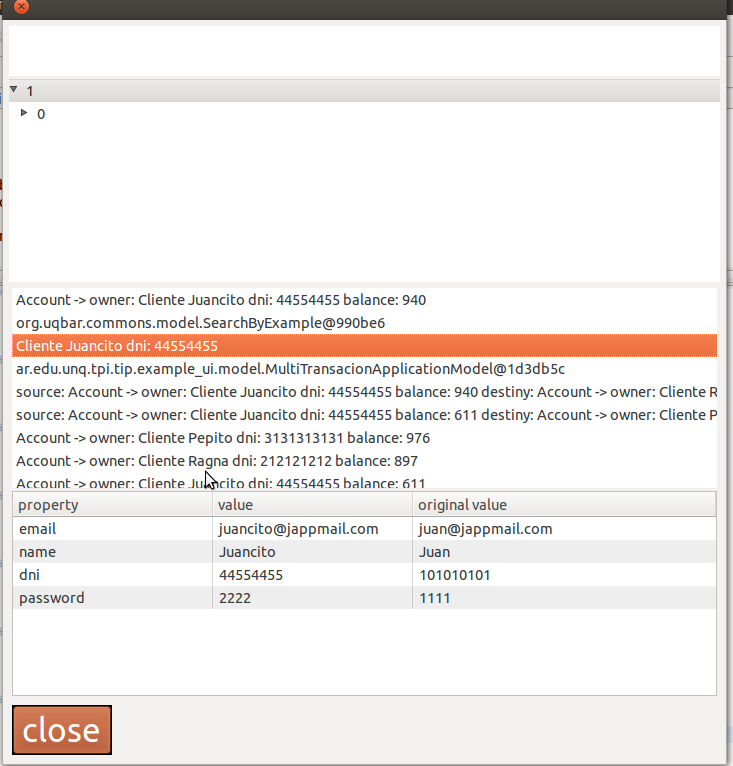
\includegraphics[width=450px, height=500px]{img/monitorTransacciones.png}
			\caption{Monitor}
			\label{monitor}
		\end{figure}	
	
	  \item[Nuevos componentes] Se agregaron algunas estructuras visuales como
	  arboles y listas.
	  \item[Bindings Anidados] Se implementaron bindings para las propiedades
	  anidadas de los objetos.
	\end{description}
